
\chapter{Performantietesten video stream}

\section{Code voor het testen van de video streams}

\begin{lstlisting}
const measureFrames = (vid, vidname) => {
  let timer = 0;
  setInterval(() => {
    timer++;
    let fps;
    if (vid) {
      fps = vid.webkitDecodedFrameCount / timer;
      const _stats = { ...stats };
      if (vidname === "yourVid") {
        _stats.yourVid.fps = fps;
        _stats.yourVid.dropped = vid.webkitDroppedFrameCount;
        _stats.yourVid.resolution = `${vid.videoWidth}x${vid.videoHeight}`;
      } else {
        _stats.receivingVid.fps = fps;
        _stats.receivingVid.dropped = vid.webkitDroppedFrameCount;
        _stats.receivingVid.resolution = `${vid.videoWidth}x${vid.videoHeight}`;
      }
      _stats.timePassed = timer;
      setStats(_stats);
    }
  }, 1000);
};
\end{lstlisting}

\section{Screenshots van de resultaten}
\begin{figure}[H]
	\centering
	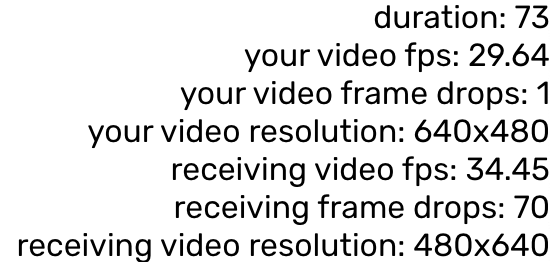
\includegraphics[width=120mm]{./img/statsPWA}		
	\caption{statistieken proof-of-concept}
\end{figure}

\begin{figure}[H]
	\centering
	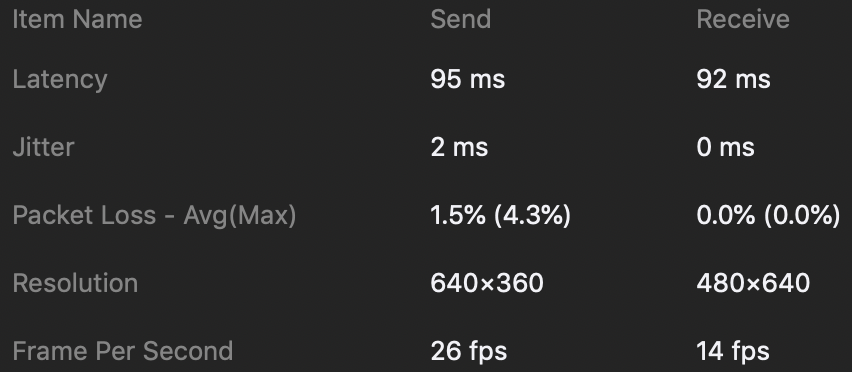
\includegraphics[width=120mm]{./img/statsZoom}		
	\caption{statistieken zoom}
\end{figure}